\subsection{Patrones de arquitectura}

\subsubsection{Arquitectura orientada a servicios}

La arquitectura orientada a servicios \cite{soa} es un estilo de arquitectura caracterizado por la orientación de servicios en servidores web. Un servicio es una unidad autónoma de una o más funciones del software diseñado para realizar una tarea específica, como recuperar información o la ejecución de operaciones.
\\

Además, la arquitectura orientada a servicios tiene como ventaja el establecimiento de una alta interoperabilidad. Esto se debe a que los entornos SOA ({\it Service Oriented Architecture}) carecen de sentido individual, pues normalmente se trata de un conjunto de servicios, creando sistemas heterogéneos. Como consecuencia de esto, existe una fácil escalabilidad y mantenimiento, ya se cada servicio se implementa por separado.
\\

Otra de las ventajas que permite es que se pueden utilizar lenguajes de programación completamente diferentes en el lado del cliente y en el servidor al realizar llamadas HTTP. Esto no ocurre, por ejemplo, en el caso de los {\it Servlets} \cite{servlet} o {\it Django} \cite{django}, donde la página web se genera en JAVA o Python respectivamente, limitándolos a utilizar un único lenguaje de programación.

\subsubsection{Arquitectura SPA}

\begin{figure}[H]
\centerline{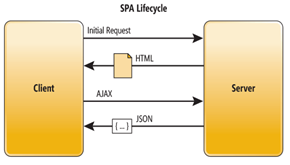
\includegraphics[width=7cm]{figuras/diseño/arquitecturaspa.png}}
\caption{Patrón de arquitectura SPA.}
\label{enlaceSPA}
\end{figure}

La arquitectura SPA ({\it Single Page Application}) \cite{spa}, reflejada en la \hyperref[enlaceSPA]{Figura 3.5}, es conocida por realizar la navegación desde el lado del cliente, mientras que el navegador no se recarga durante su uso. 
\\

Una de las principales ventajas que tiene con respecto a las aplicaciones tradicionales es que permite realizar cualquier aplicación de escritorio vía web, siendo el tiempo de respuesta mucho más rápido. Esto es así porque no tiene que ir a buscar continuamente la información al servidor. Además, se reduce la carga del servidor al realizar todas las operaciones sobre el cliente. Al generarse la aplicación en el navegador web, solo es necesario ir llamando a la API cuando se necesita hacer uso del servidor.